% Options for packages loaded elsewhere
\PassOptionsToPackage{unicode}{hyperref}
\PassOptionsToPackage{hyphens}{url}
%
\documentclass[
  ignorenonframetext,
  aspectratio=169]{beamer}
\usepackage{pgfpages}
\setbeamertemplate{caption}[numbered]
\setbeamertemplate{caption label separator}{: }
\setbeamercolor{caption name}{fg=normal text.fg}
\beamertemplatenavigationsymbolsempty
% Prevent slide breaks in the middle of a paragraph
\widowpenalties 1 10000
\raggedbottom
\setbeamertemplate{part page}{
  \centering
  \begin{beamercolorbox}[sep=16pt,center]{part title}
    \usebeamerfont{part title}\insertpart\par
  \end{beamercolorbox}
}
\setbeamertemplate{section page}{
  \centering
  \begin{beamercolorbox}[sep=12pt,center]{part title}
    \usebeamerfont{section title}\insertsection\par
  \end{beamercolorbox}
}
\setbeamertemplate{subsection page}{
  \centering
  \begin{beamercolorbox}[sep=8pt,center]{part title}
    \usebeamerfont{subsection title}\insertsubsection\par
  \end{beamercolorbox}
}
\AtBeginPart{
  \frame{\partpage}
}
\AtBeginSection{
  \ifbibliography
  \else
    \frame{\sectionpage}
  \fi
}
\AtBeginSubsection{
  \frame{\subsectionpage}
}
\usepackage{lmodern}
\usepackage{amssymb,amsmath}
\usepackage{ifxetex,ifluatex}
\ifnum 0\ifxetex 1\fi\ifluatex 1\fi=0 % if pdftex
  \usepackage[T1]{fontenc}
  \usepackage[utf8]{inputenc}
  \usepackage{textcomp} % provide euro and other symbols
\else % if luatex or xetex
  \usepackage{unicode-math}
  \defaultfontfeatures{Scale=MatchLowercase}
  \defaultfontfeatures[\rmfamily]{Ligatures=TeX,Scale=1}
\fi
\usetheme[]{Frankfurt}
\usecolortheme{beaver}
% Use upquote if available, for straight quotes in verbatim environments
\IfFileExists{upquote.sty}{\usepackage{upquote}}{}
\IfFileExists{microtype.sty}{% use microtype if available
  \usepackage[]{microtype}
  \UseMicrotypeSet[protrusion]{basicmath} % disable protrusion for tt fonts
}{}
\makeatletter
\@ifundefined{KOMAClassName}{% if non-KOMA class
  \IfFileExists{parskip.sty}{%
    \usepackage{parskip}
  }{% else
    \setlength{\parindent}{0pt}
    \setlength{\parskip}{6pt plus 2pt minus 1pt}}
}{% if KOMA class
  \KOMAoptions{parskip=half}}
\makeatother
\usepackage{xcolor}
\IfFileExists{xurl.sty}{\usepackage{xurl}}{} % add URL line breaks if available
\IfFileExists{bookmark.sty}{\usepackage{bookmark}}{\usepackage{hyperref}}
\hypersetup{
  pdftitle={Tissue culture techniques},
  pdfauthor={Deependra Dhakal},
  hidelinks,
  pdfcreator={LaTeX via pandoc}}
\urlstyle{same} % disable monospaced font for URLs
\newif\ifbibliography
\setlength{\emergencystretch}{3em} % prevent overfull lines
\providecommand{\tightlist}{%
  \setlength{\itemsep}{0pt}\setlength{\parskip}{0pt}}
\setcounter{secnumdepth}{-\maxdimen} % remove section numbering
\usepackage{tikz}
\usepackage[absolute,overlay]{textpos}
\usepackage{pdfrender}

% % set titlepage in a TikZ node for modifications
\setbeamertemplate{title page}{%
\begin{tikzpicture}[remember picture,overlay]
\fill[blue]
  ([yshift=15pt]current page.west) rectangle (current page.south east);
\node[anchor=east] 
  at ([yshift=-50pt]current page.north east) (author)
  {\parbox[t]{.6\paperwidth}{\raggedleft%
    \usebeamerfont{author}\textcolor{orange}{%
    \textpdfrender{
    TextRenderingMode=FillStroke,
    FillColor=orange,
    LineWidth=.1ex,
    }{\insertauthor}}}};
\node[anchor=north east] 
  at ([yshift=-70pt]current page.north east) (institute)
  {\parbox[t]{.78\paperwidth}{\raggedleft%
    \usebeamerfont{institute}\textcolor{gray}{\insertinstitute}}};
\node[anchor=south west] 
  at ([yshift=-120pt]current page.west) (logo)
  {\parbox[t]{.20\paperwidth}{\raggedleft%
    \usebeamercolor[fg]{titlegraphic}\inserttitlegraphic}};
\node[anchor=east]
  at ([yshift=-30pt,xshift=-20pt]current page.east) (title)
  {\parbox[t]{\textwidth}{\raggedleft%
 \usebeamerfont{author}\textcolor{white}{%
    \textpdfrender{
    TextRenderingMode=FillStroke,
    FillColor=white,
    LineWidth=.25ex,
    LineJoinStyle=1,
    Flatness=20,
    RenderingIntent=Perceptual,
    }{\inserttitle}}}};
\node[anchor=east]
  at ([yshift=-60pt,xshift=-20pt]current page.east) (subtitle)
  {\parbox[t]{.5\paperwidth}{\raggedleft\usebeamerfont{subtitle}\textcolor{black}{\insertsubtitle}}};
\end{tikzpicture}
}
\titlegraphic{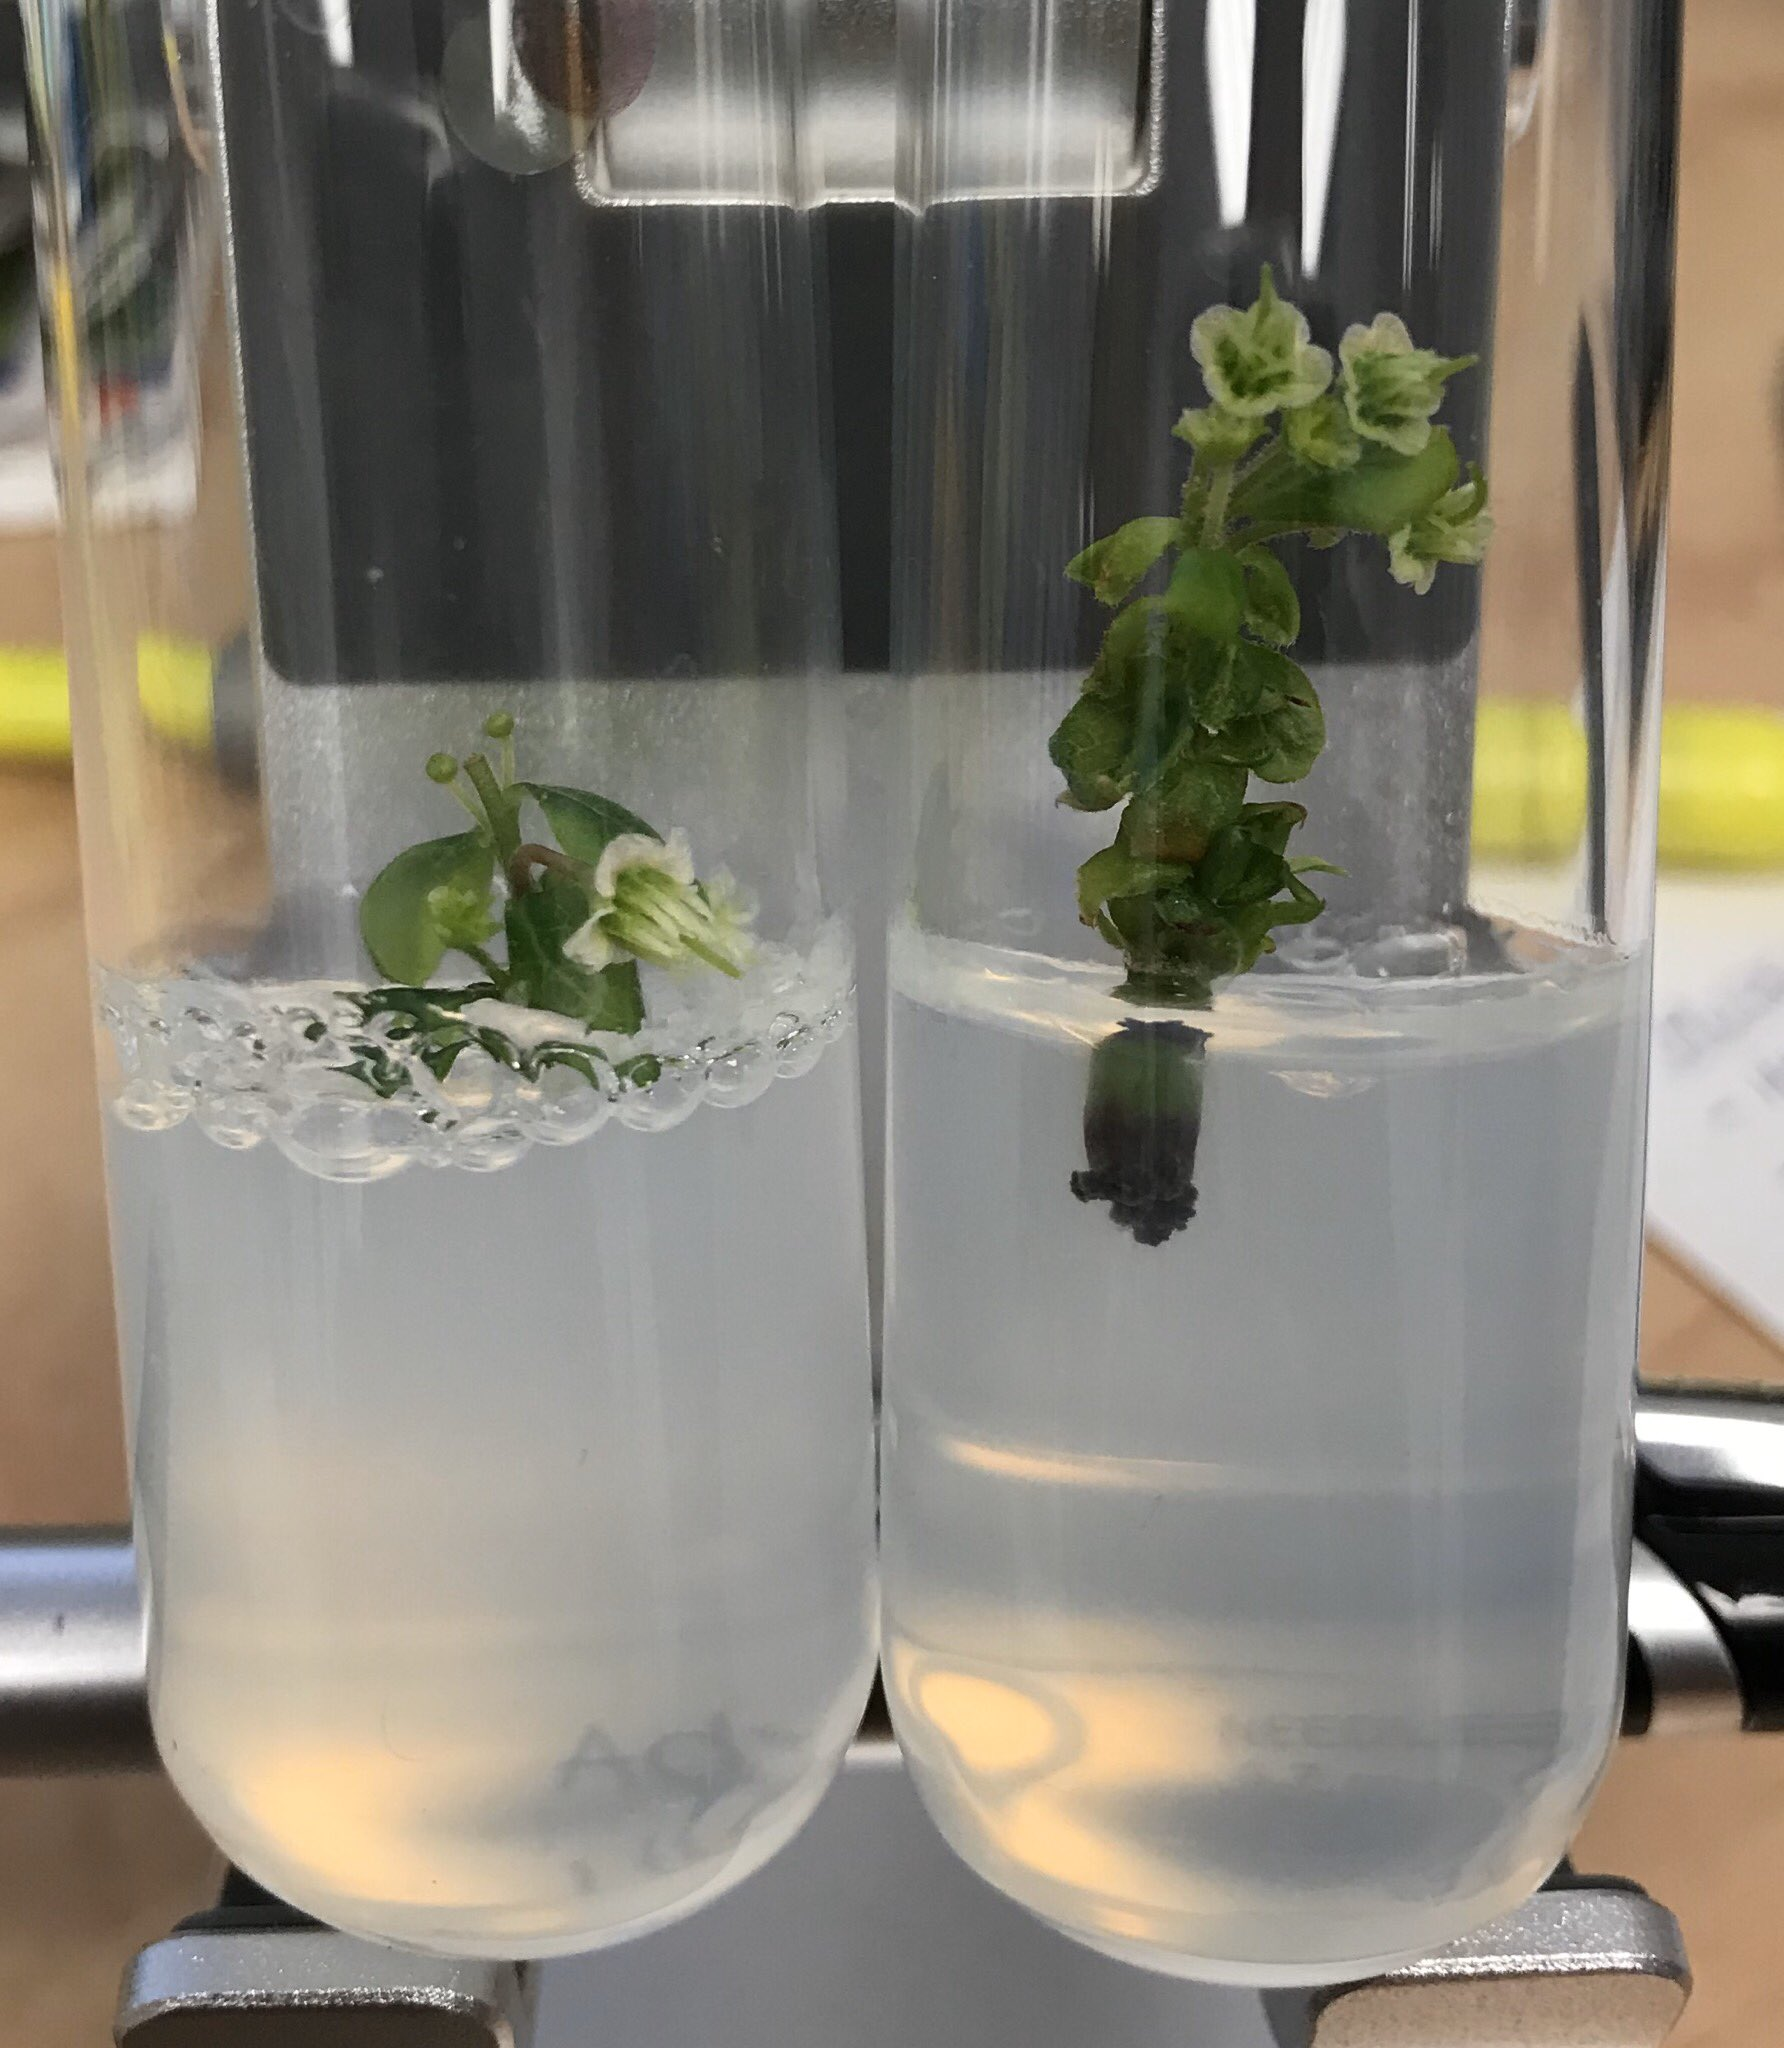
\includegraphics[width=7cm]{04-tissue_culture_techniques_vaccinium-plant.jpeg}}

% % set background image if you will
% \usebackgroundtemplate%
% {%
%     \includegraphics[width=\paperwidth,height=\paperheight]{02-dna_modification_background_dna_helix.jpg}%
% }

% % set caption font size
% % note that beamer presentation native captions have their own configs
% \usepackage{caption}
% \captionsetup{font=footnotesize}

% this font option is amenable for beamer
\setbeamerfont{caption}{size=\tiny}

% some beamer themes naturally might not support navigation symbols
% \setbeamertemplate{navigation symbols}{} % remove navigation symbols

\setbeamertemplate{footline}[page number] % insert page number in footline

% \setbeamertemplate{navigation symbols}{slide} % insert slide indication in navigation
% \setbeamertemplate{navigation symbols}{frame} % insert frame indication in navigation
% \setbeamertemplate{navigation symbols}{section} % insert section indication in navigation
% \setbeamertemplate{navigation symbols}{subsection} % insert subsection indication in navigation

% \AtBeginSubsection{} % supress subsection display

\title{Tissue culture techniques}
\author{Deependra Dhakal}
\date{Academic year: 2022-2023}
\institute{College of Natural Resource Management, Tikapur,
Kailali \and Agriculture and Forestry University}

\begin{document}
\frame{\titlepage}

\begin{frame}[allowframebreaks]
  \tableofcontents[hideallsubsections]
\end{frame}
\hypertarget{overview}{%
\section{Overview}\label{overview}}

\begin{frame}{Background}
\protect\hypertarget{background}{}
\begin{itemize}
\tightlist
\item
  In vitro = a-xenic = sterile culture
\item
  Plant tissue culture is generally used for the aseptic culture of
  cells, tissues, organs, and their components under defined physical
  and chemical conditions in vitro.
\item
  First approach made by Henri-Louis Duhumel du Monceau in 1756
  (observed callus formation in plants)
\item
  Development of cell theory by Schleiden and Schwann during 1830s
\item
  Theoretical basis for plant tissue culture was proposed by Gottlieb
  Haberlandt in his address to the German Academy of Science in 1902 on
  his experiments on the culture of single cells.
\item
  Definition: It is a technique of growing plant cells, tissues and
  organs in an artificial prepared medium under aseptic conditions.
\end{itemize}
\end{frame}

\begin{frame}{History}
\protect\hypertarget{history}{}
\begin{itemize}
\tightlist
\item
  The first true plant tissue cultures were obtained by Gautheret (1934,
  1935) from cambial tissue of \emph{Acer pseudoplatanus}.
\item
  The first plant growth hormone indoleacetic acid (IAA) was discovered
  in the mid-1930s by F. Kogl and his coworkers.
\item
  In 1934 Professor Philip White successfully cultured tomato roots.
\item
  In 1939 Gautheret successfully cultured carrot tissue.
\item
  Later in 1955 Carlos Miller and Folke Skoog published their discovery
  of the hormone kinetin, a cytokinin.
\item
  In 1962, Toshio Murashige and Skoog published the composition a plant
  tissue culture medium known as MS (named for the first letters of
  their last names) medium.
\item
  Murashige was a doctoral student in Professor Skoog's lab, and they
  developed the now-famous MS medium working with tobacco tissue
  cultures.
\end{itemize}
\end{frame}

\begin{frame}{Some terminologies}
\protect\hypertarget{some-terminologies}{}
\begin{itemize}
\tightlist
\item
  Dedifferentiation: The phenomenon of mature cells reverting to a
  meristematic state and forming undifferentiated callus tissues.
\item
  Redifferentiation: The ability of the component cells of the callus to
  differentiate into a whole plant or a plant organ is termed as
  redifferentiation.
\item
  Cellular totipotency: These two phenomena of dedifferentiation and
  redifferentiation are inherent in the capacity of a plant cell, and
  thus giving rise to a whole plant in known as cellular totipotency.
\end{itemize}
\end{frame}

\begin{frame}{Basic steps}
\protect\hypertarget{basic-steps}{}
\begin{itemize}
\tightlist
\item
  Select the source of explant
\item
  Trimming
\item
  Several washes in running water
\item
  Surface sterilization
\item
  Basic sterilization
\item
  Preparation of culture media
\item
  Culture in a good environmental condition
\item
  Sub culture, if necessary
\item
  Plant regeneration, hardening and transfer to soil
\end{itemize}
\end{frame}

\hypertarget{tissue-culture-laboratory-setup}{%
\section{Tissue culture laboratory
setup}\label{tissue-culture-laboratory-setup}}

\begin{frame}{}
\protect\hypertarget{section}{}
\begin{center}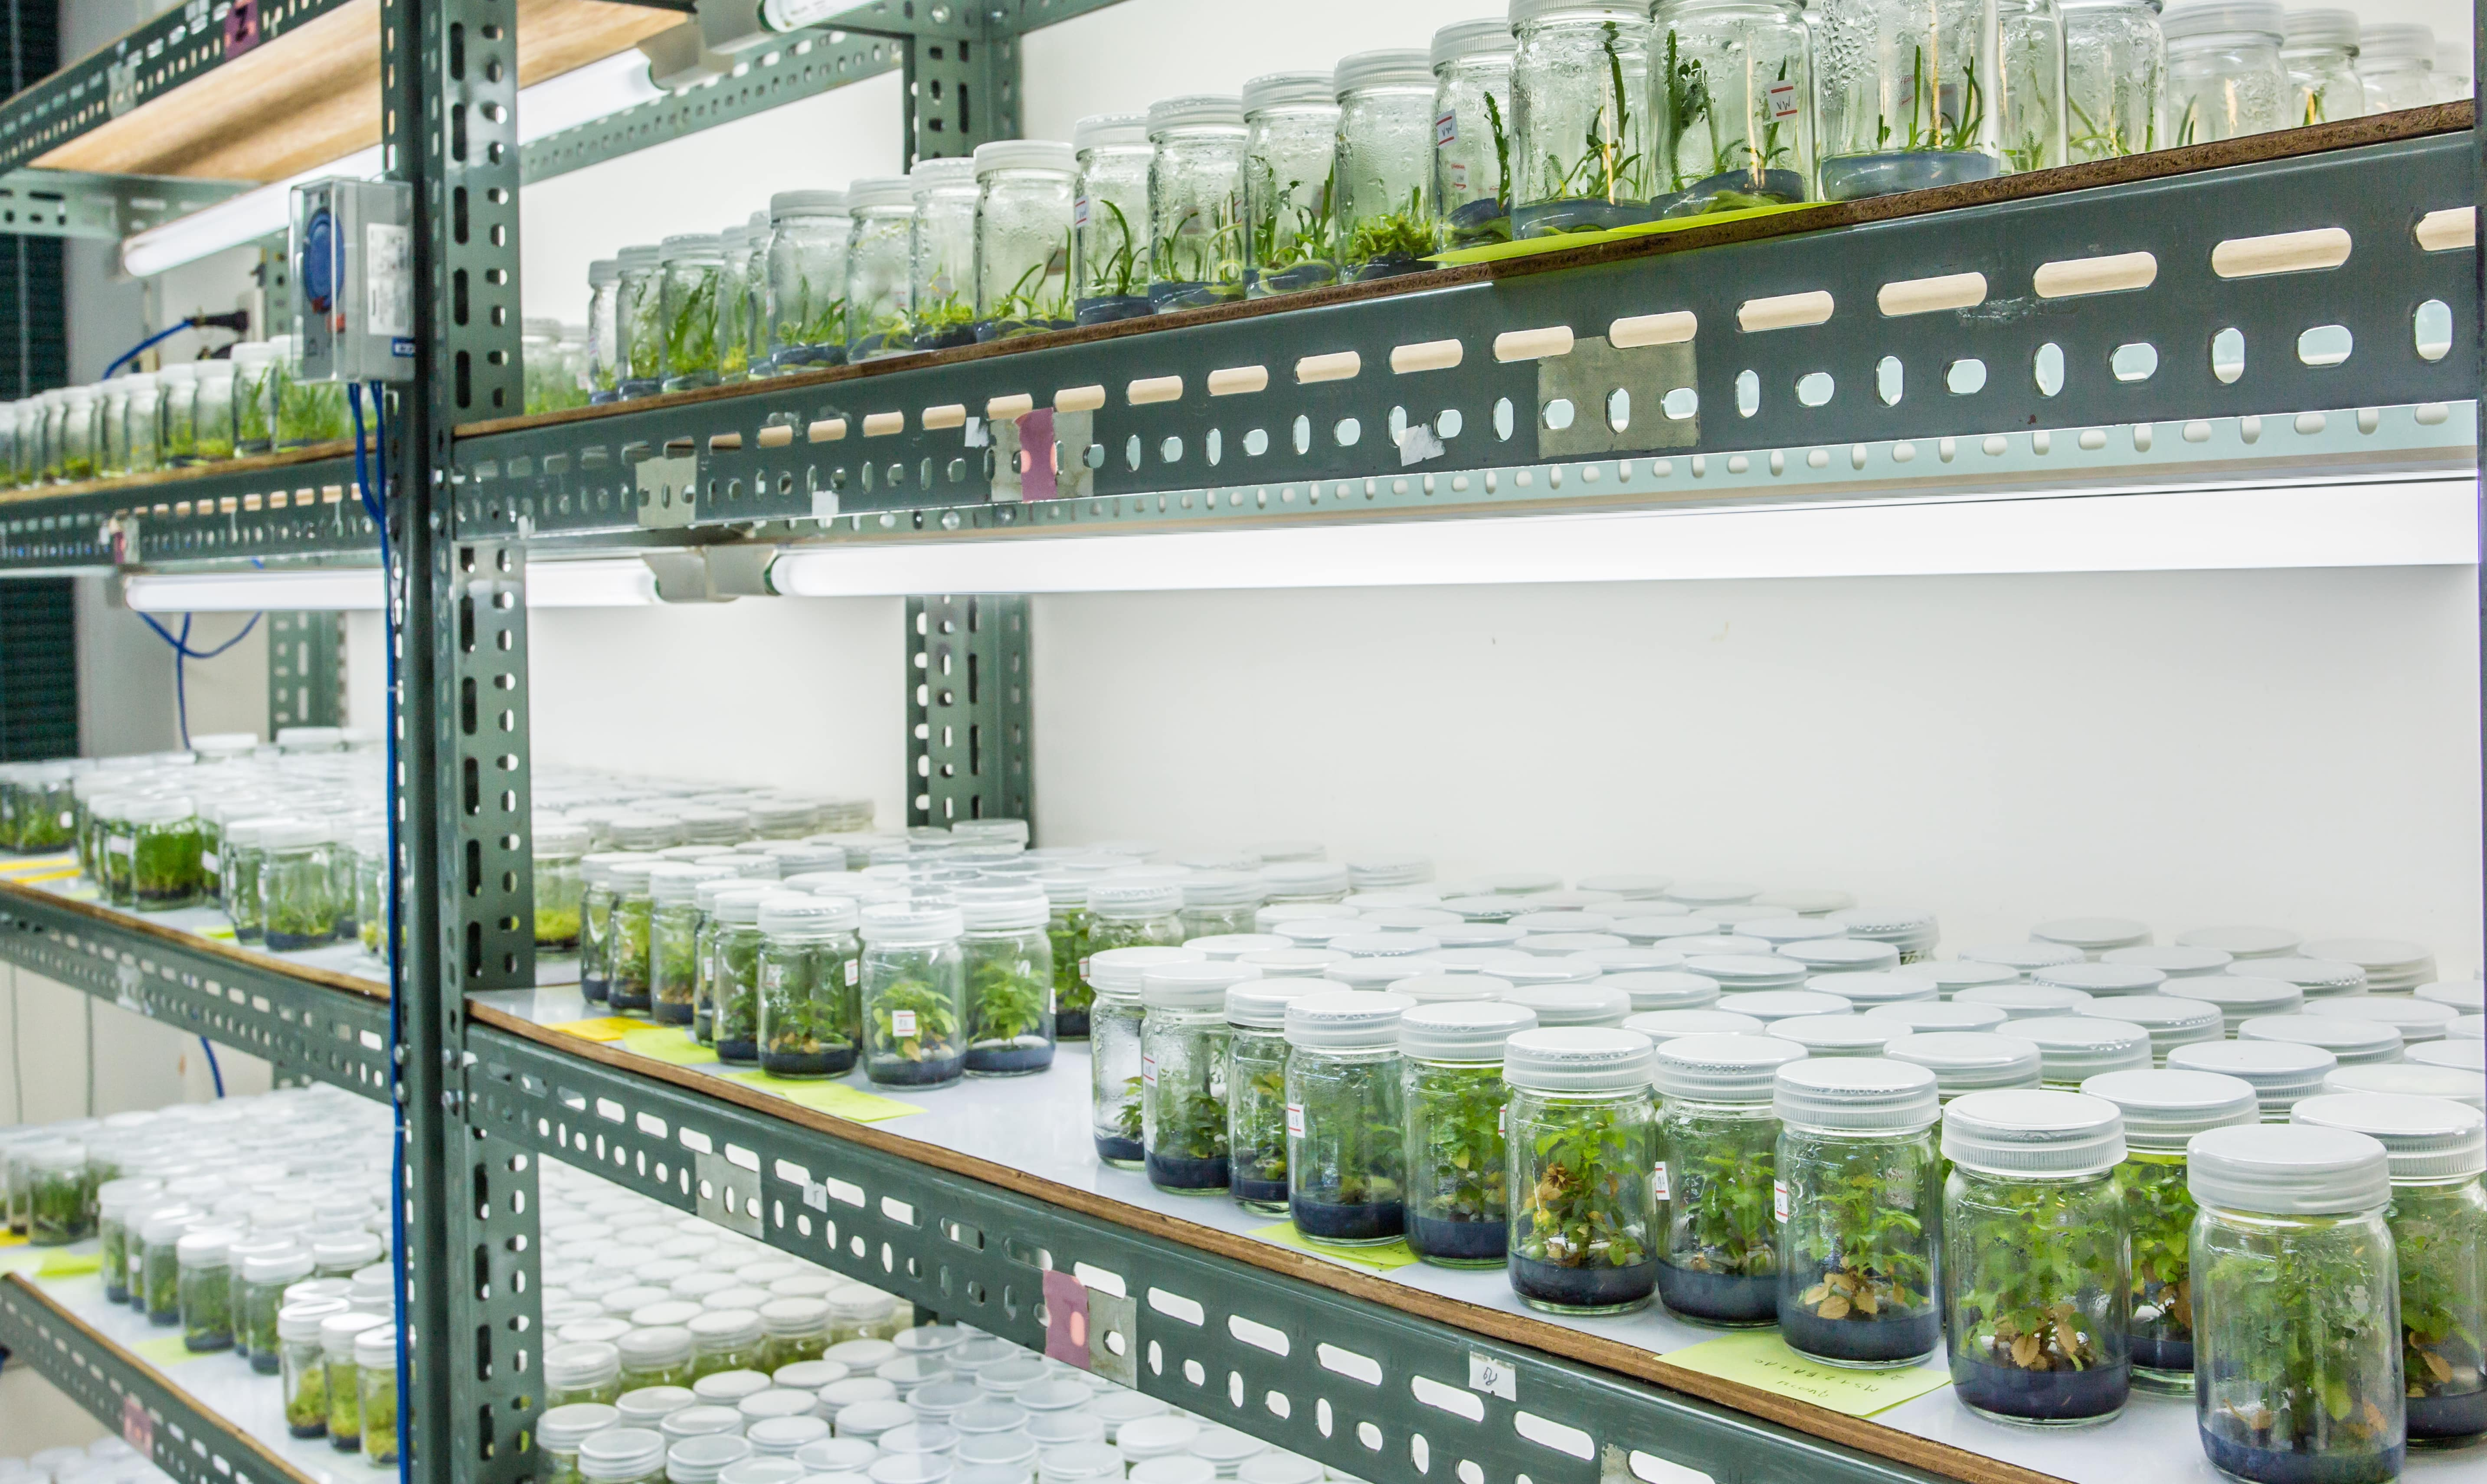
\includegraphics[width=0.98\linewidth]{../images/tissue-culture-equipments} \end{center}
\end{frame}

\begin{frame}{}
\protect\hypertarget{section-1}{}
\begin{columns}[T,onlytextwidth]
  \column{0.5\textwidth}

\begin{figure}
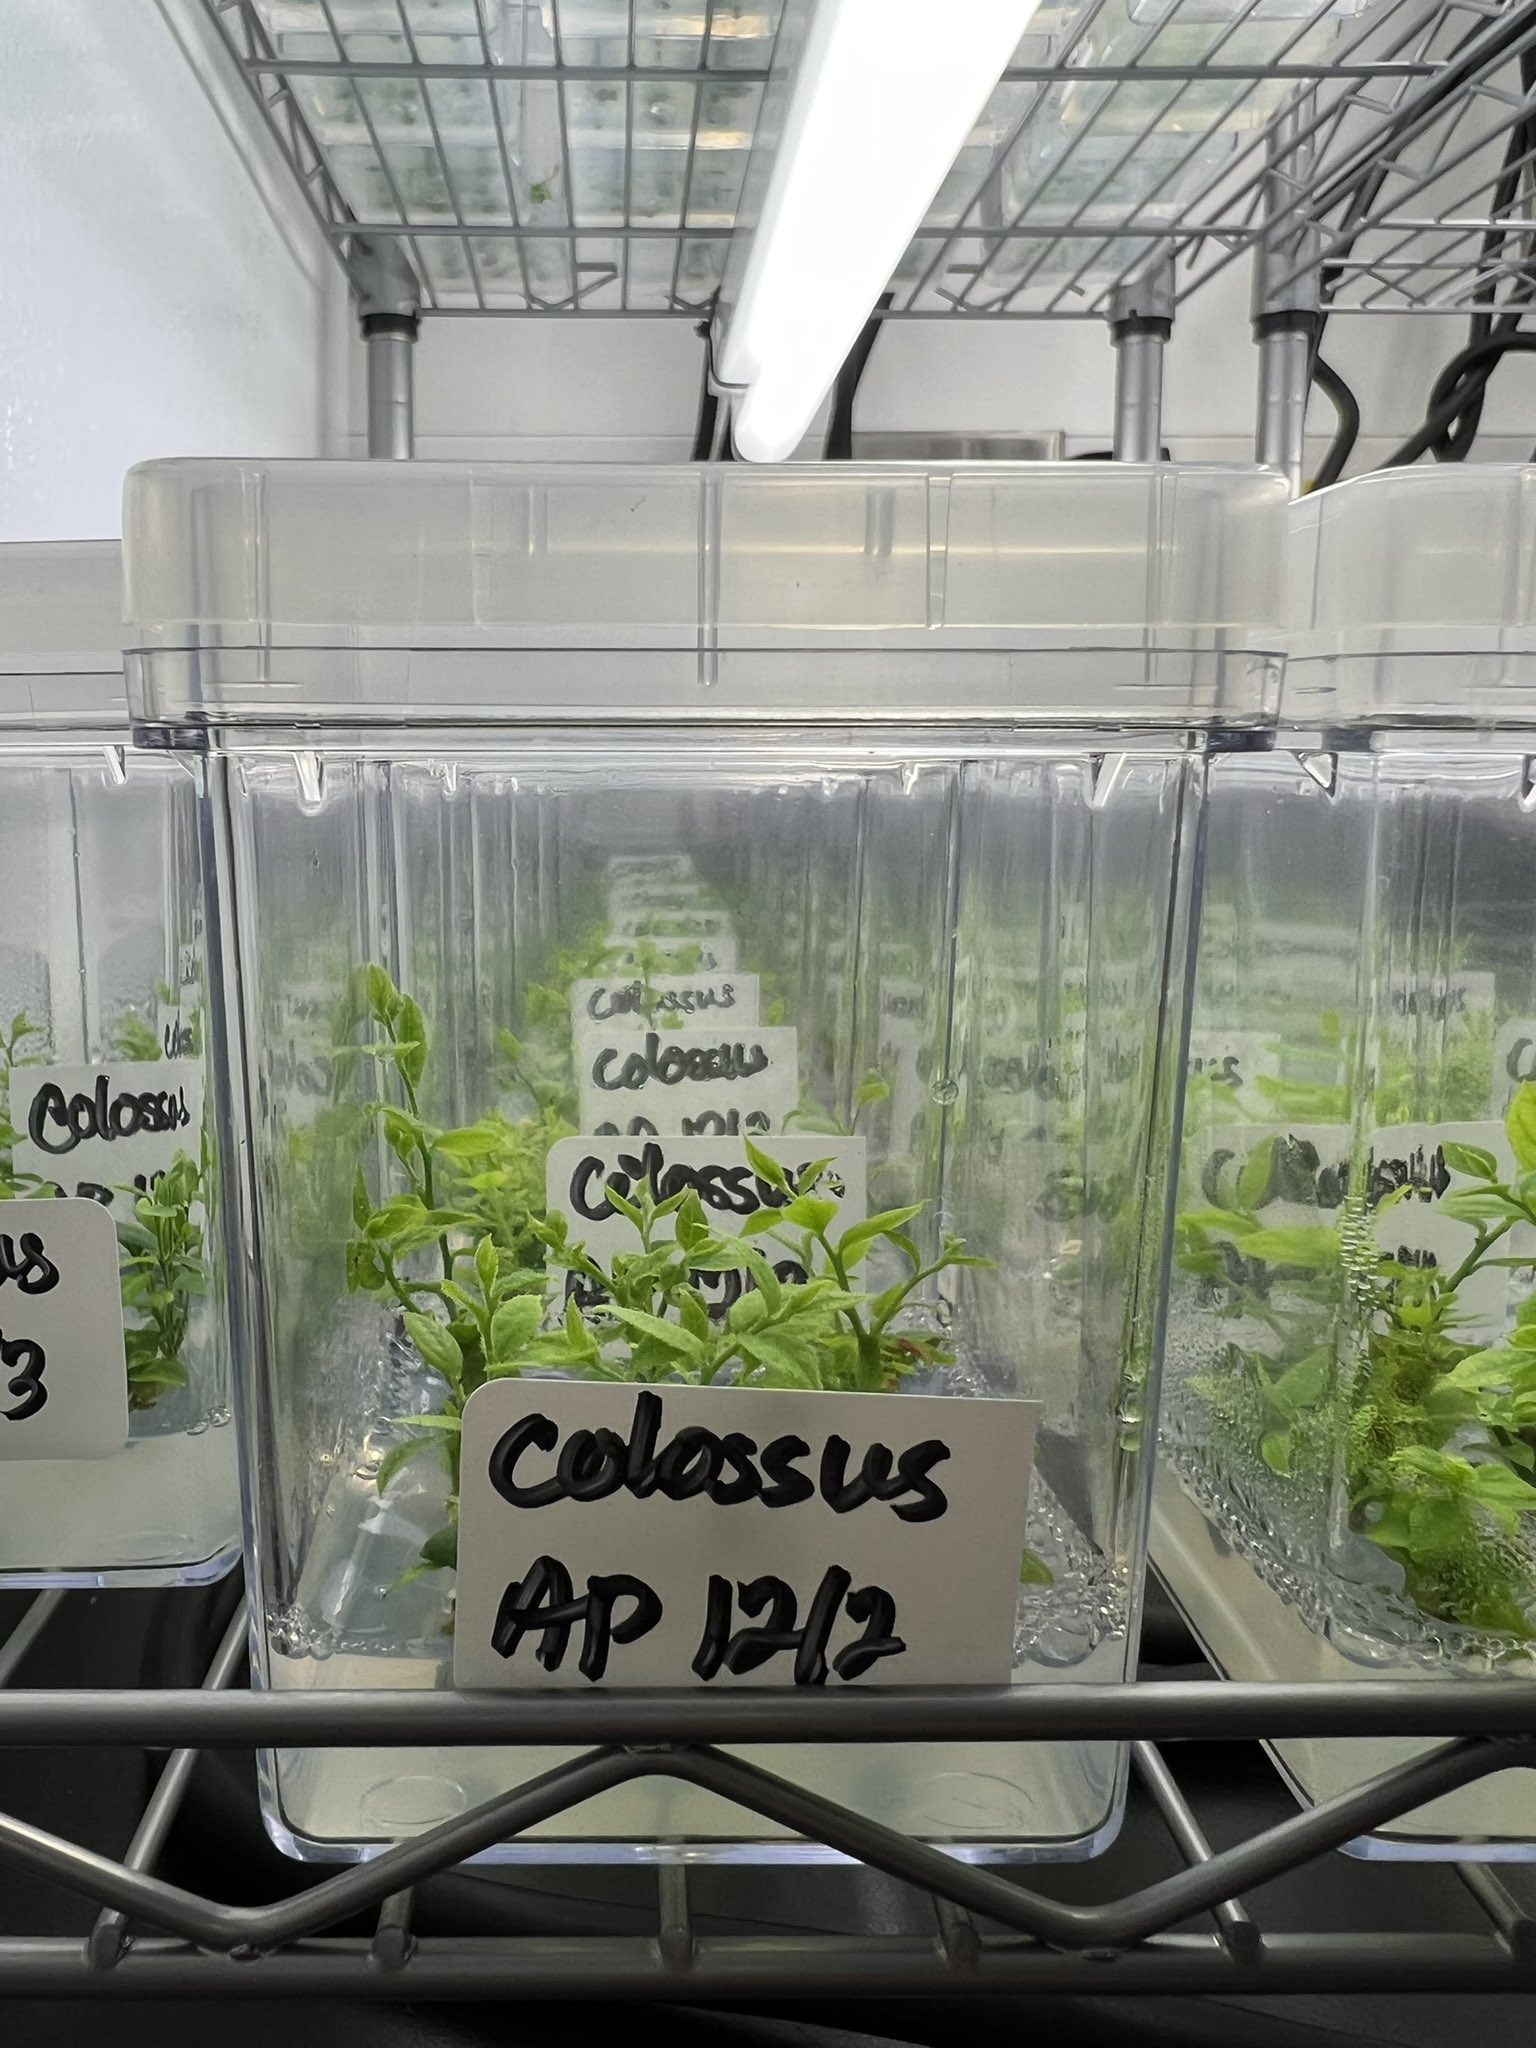
\includegraphics[width=0.7\linewidth]{../images/blueberry-propagation} \caption{Blueberry micropropagation container}\label{fig:blueberry-propagation-media}
\end{figure}

  \column{0.5\textwidth}


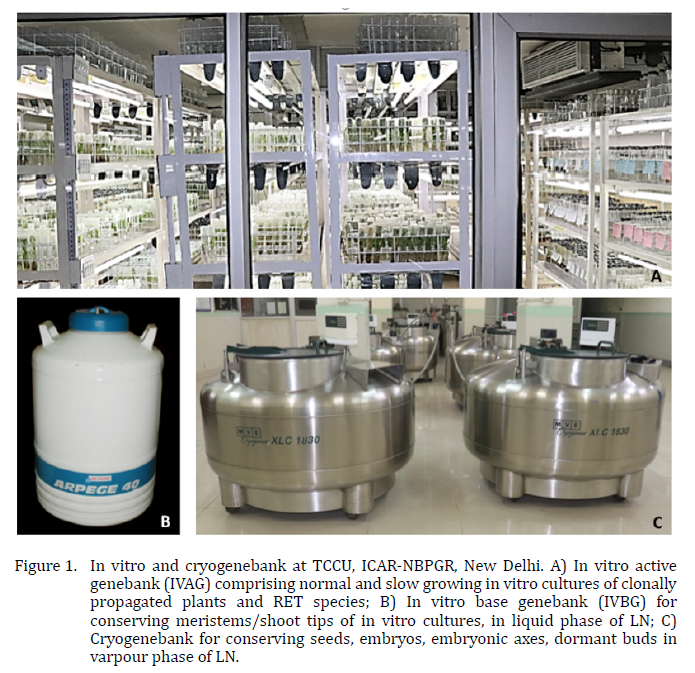
\includegraphics[width=0.8\linewidth]{../images/invitro-gene-banks} 

\end{columns}
\end{frame}

\begin{frame}{Media preparations/culture evaluation}
\protect\hypertarget{media-preparationsculture-evaluation}{}
\begin{columns}[T,onlytextwidth]
  \column{0.5\textwidth}
  \begin{itemize}

  \item Bench
  \item Gas outlet
  \item Hot plate and magnetic stirrer
  \item Analytical and top-loading balances
  \item pH meter
  \item Refrigerator, freezer
  \item Water purification and storage system
  \item Dish-washing area
  \end{itemize}

  \column{0.5\textwidth}

  \begin{itemize}

  \item Storage facilities-glassware, chemicals
  \item Autoclave (pressure-cooker will work for small media volume)
  \item Low bench with inverted light and dissecting microscopes (avoid locating next autoclaves or other high-humidity areas)
  \item Fume hood
  \item Desk and file cabinets
  \item Desktop centrifuge, spectrophotometer, microwave (transformation studies and protoplast isolation)

  \end{itemize}

\end{columns}
\end{frame}

\begin{frame}{Aseptic transfer area}
\protect\hypertarget{aseptic-transfer-area}{}
\begin{enumerate}
\tightlist
\item
  Laminar air flow transfer hood and comfortable chair
\item
  Dissecting microscope
\item
  Gas outlet
\item
  Vacuum lines
\item
  Forceps, spatulas, scalpel, and disposable blades
\end{enumerate}
\end{frame}

\begin{frame}{Laminar flow cabinet and units}
\protect\hypertarget{laminar-flow-cabinet-and-units}{}
\begin{columns}[T,onlytextwidth]
  \column{0.4\textwidth}

\begin{figure}
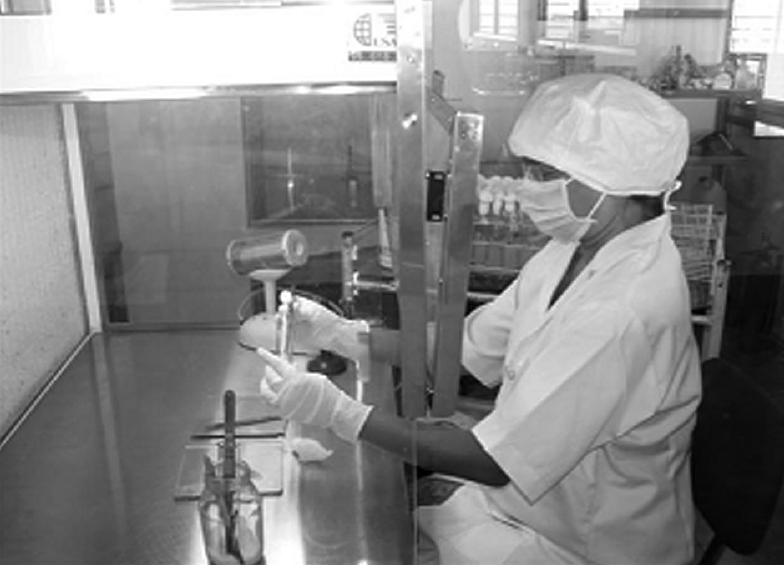
\includegraphics[width=0.8\linewidth]{../images/working_laminar_flow_hood} \caption{Working in the laminar flow hood}\label{fig:aseptic-transfer}
\end{figure}

  \begin{itemize}
  \scriptsize
  \item Air purification system
  \item HEPA (High efficiency particulate air) filter
  \item Stainless steel working board
  \item Air blower
  \item UV lamp
  \item Safety glasses
  \end{itemize}

  \column{0.6\textwidth}


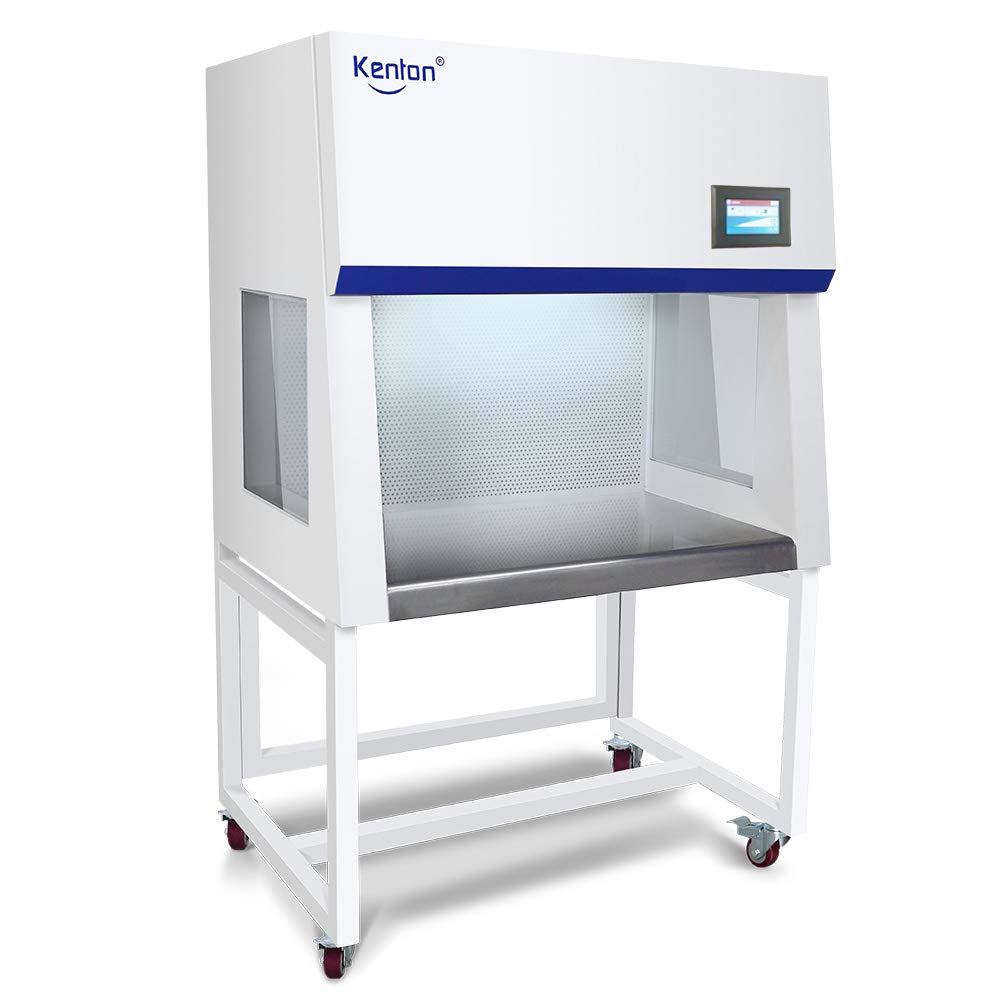
\includegraphics[width=0.8\linewidth]{../images/laminar-hood} 
  
\end{columns}
\end{frame}

\begin{frame}{Environmentally Controlled Culture Area}
\protect\hypertarget{environmentally-controlled-culture-area}{}
\begin{enumerate}
\tightlist
\item
  Shelves with lighting on a timer and controlled temperature
\item
  Incubators---with controlled temperature and light
\item
  Orbital shakers
\end{enumerate}
\end{frame}

\begin{frame}{Conditions}
\protect\hypertarget{conditions}{}
\begin{itemize}
\tightlist
\item
  High humidity in culture room should be avoided.
\item
  Most cultures can be incubated at \(25-27~^\circ C\) under a 16:8-h
  light:dark photoperiod controlled by clock timers.
\item
  Light conditions can be manipulated by mounted fluorescent lamps with
  light readings (by quantum radiometer-photometer) of 40-200 foot
  candles (full sun is approximately 10000 foot candles).
\end{itemize}
\end{frame}

\hypertarget{basal-media-components-and-preparation}{%
\section{Basal media components and
preparation}\label{basal-media-components-and-preparation}}

\begin{frame}{Basal media components and preparation}
\begin{itemize}
\tightlist
\item
  No single medium will support the growth of all cells.
\item
  Literature serves best to the purpose, else suitable medium is based
  on trial and error.
\item
  Medium contains in general, inorganic salts, and organic compounds
  like plant growth regulators, vitaims, a carbohydrate, hexitols, and a
  gelling agent.
\item
  Iron stably provided in chelated form with EDTA.
\item
  Medium can also include amino acids, antibiotics, or natural
  complexes.
\item
  Sometimes cultures are grown in the dark and do not photosynthesize at
  all.
\item
  Most media are adjusted to a pH of 5.2-5.8.
\item
  Solidification is done using agar derived from seaweed or agar
  substitutes such as \(Gelrite^{TM}\) or \(Phytagel^{TM}\).
\item
  Woody Plant Medium (WPM) is suitable for culturing trees.
\end{itemize}
\end{frame}

\begin{frame}{Inorganic salts}
\protect\hypertarget{inorganic-salts}{}
\begin{itemize}
\tightlist
\item
  The Murashige and Skoog (MS) (1962) formulation is the most widely
  used formulation.
\item
  The MS formulation was developed to insure that no increases in cell
  growth in vitro were due to the introduction of additional salts from
  plant tissue extracts which were being tested at that time.
\item
  The MS formulation insured that the inorganic nutrients were not
  limiting to tobacco cell growth and organic supplements such as yeast
  extract, coconut milk, casein hydrolysate, and plant extracts were no
  longer essential sources of the inorganic salts.
\end{itemize}
\end{frame}

\begin{frame}{}
\protect\hypertarget{section-2}{}
\begin{itemize}
\tightlist
\item
  The distinguishing feature of the MS inorganic salts is their high
  content of nitrate, potassium, and ammonium in comparison to other
  salt formulations.
\item
  These salt stocks are prepared at 100 times the final medium
  concentration, and each stock is added at the rate of 10 ml per 1000
  ml of medium prepared. The NaFeEDTA stock should be protected from
  light by storing it in a bottle that is amber colored or wrapped in
  aluminum foil. Concentrated salt stocks enhance the accuracy and speed
  of media preparation.
\item
  Salt stocks are best stored in refrigerator and are stable for several
  months.
\end{itemize}
\end{frame}

\begin{frame}{}
\protect\hypertarget{section-3}{}
\begin{figure}
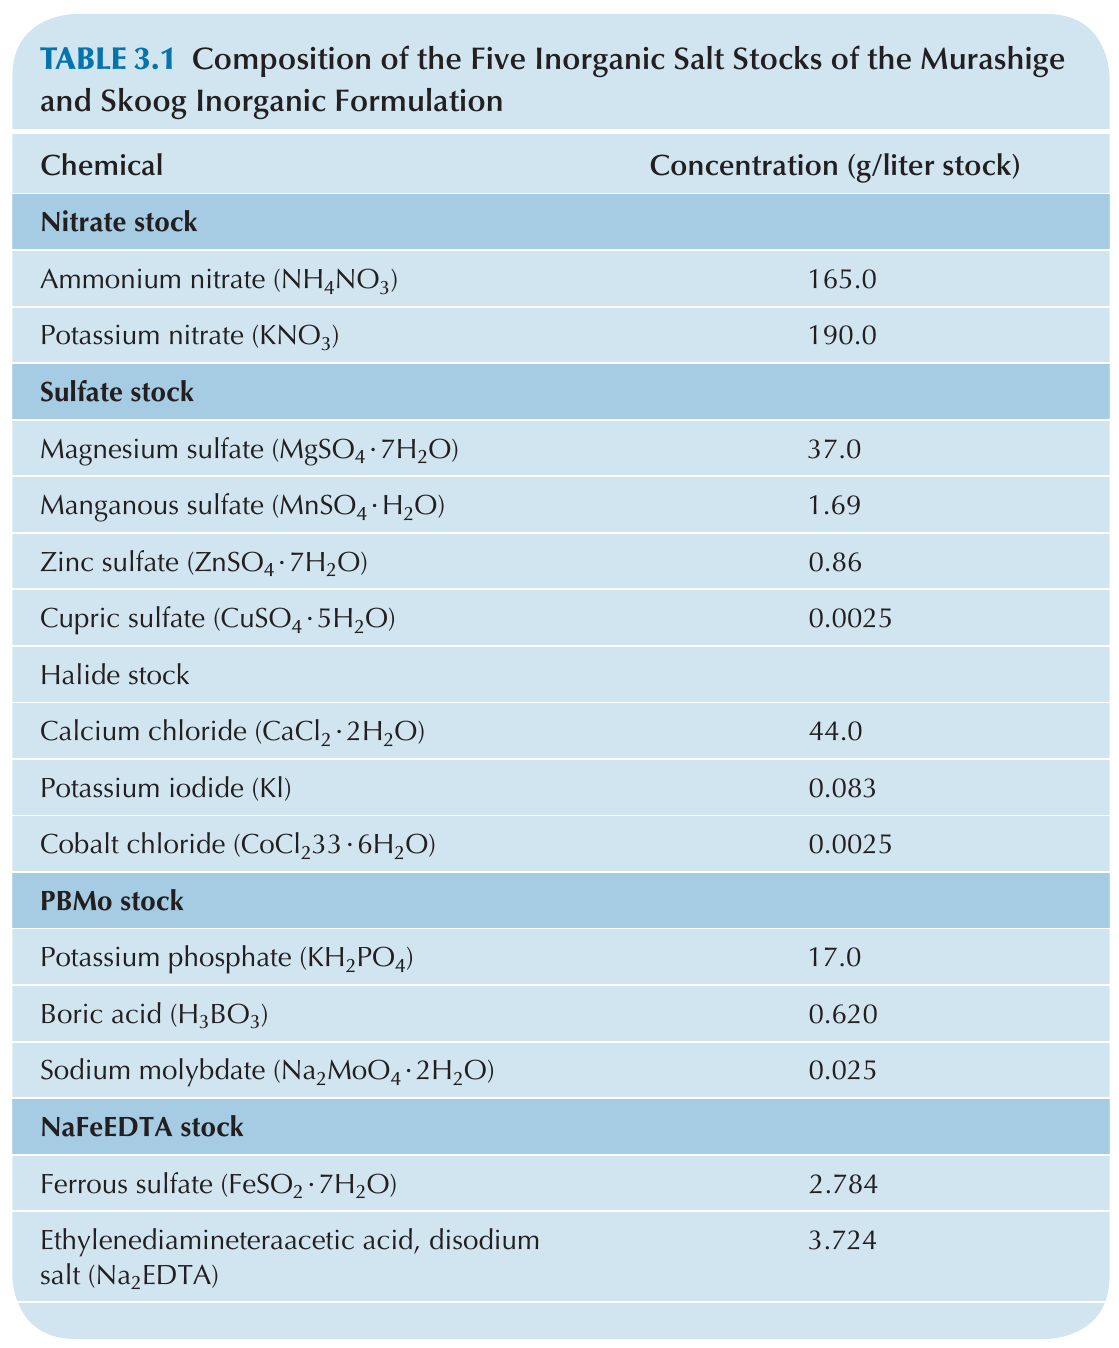
\includegraphics[width=0.38\linewidth]{../images/inorganic_salt_ms} \caption{Composition of the five inorganic salt stocks of the Murashige and Skoog Inorganic formulation}\label{fig:inorganic-salts}
\end{figure}
\end{frame}

\begin{frame}{}
\protect\hypertarget{section-4}{}
\begin{figure}
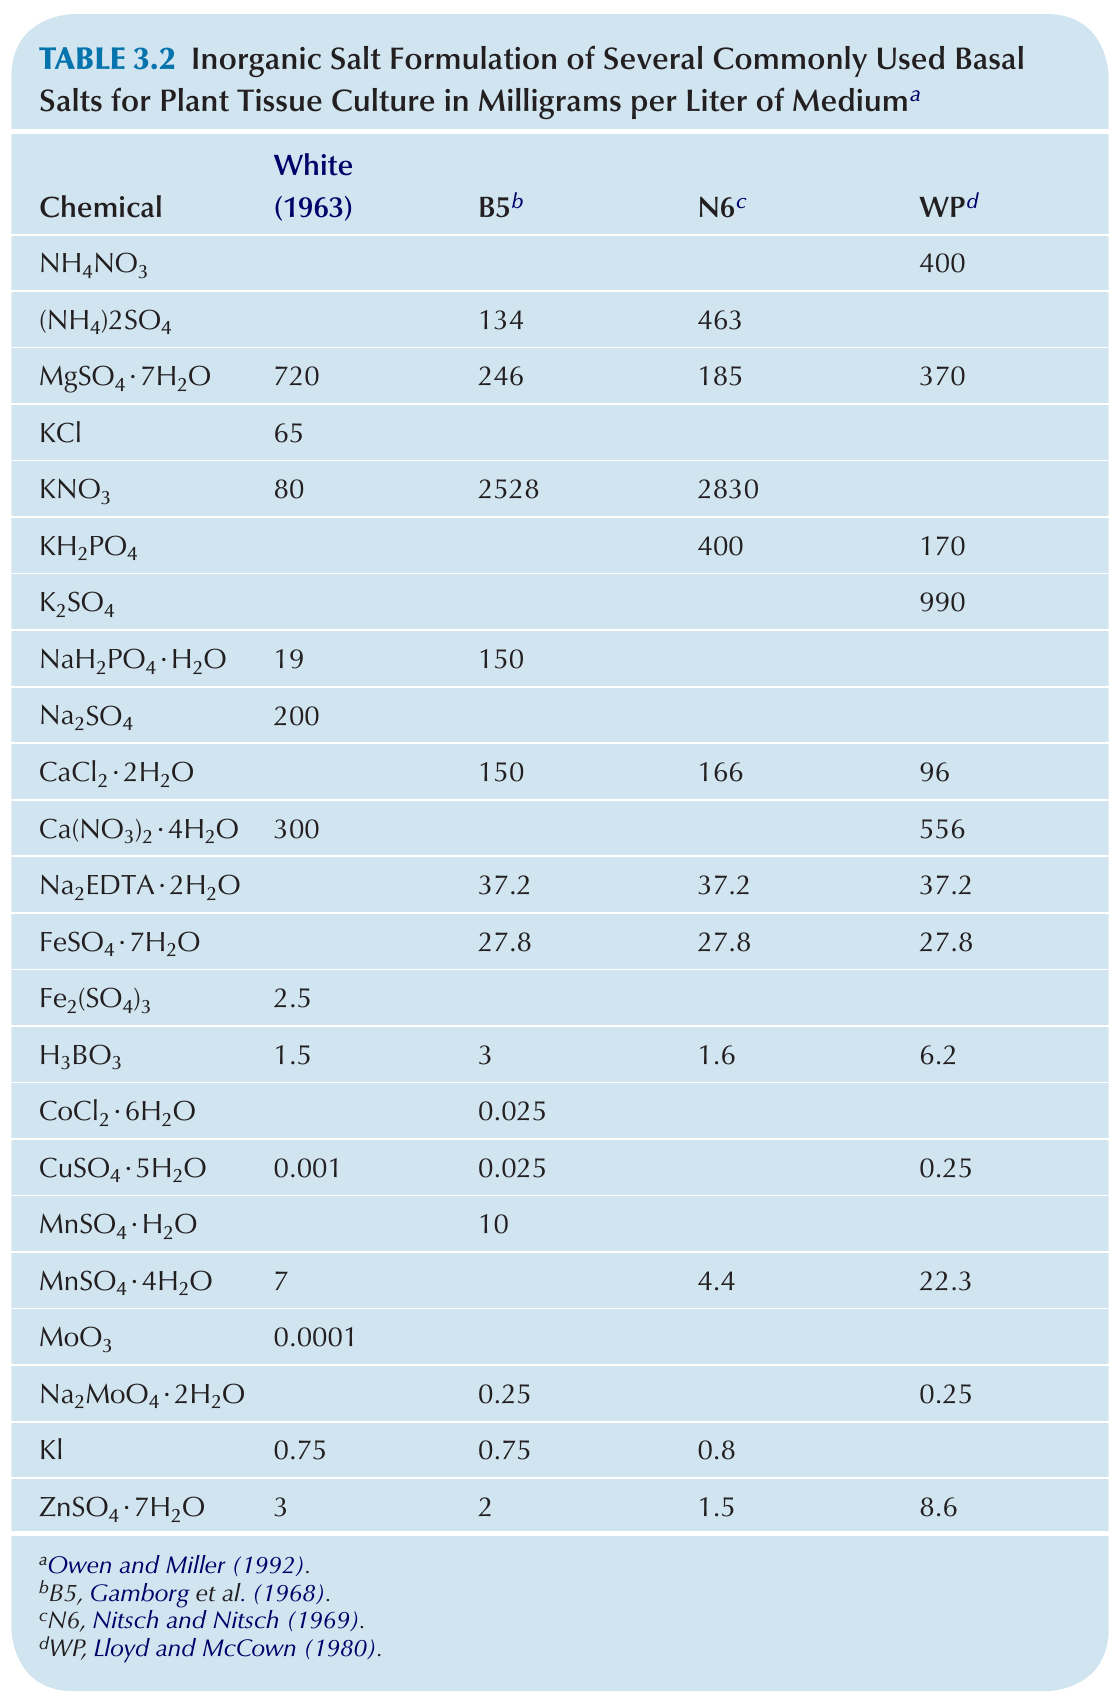
\includegraphics[width=0.35\linewidth]{../images/is_formulation_mediums} \caption{Inorganic Salt Formulation of Several Commonly Used Basal Salts for Plant Tissue Culture in Milligrams per Liter of Medium}\label{fig:is-formulation}
\end{figure}
\end{frame}

\begin{frame}{Growth regulators}
\protect\hypertarget{growth-regulators}{}
\begin{columns}[T,onlytextwidth]
  \column{0.5\textwidth}

\begin{figure}
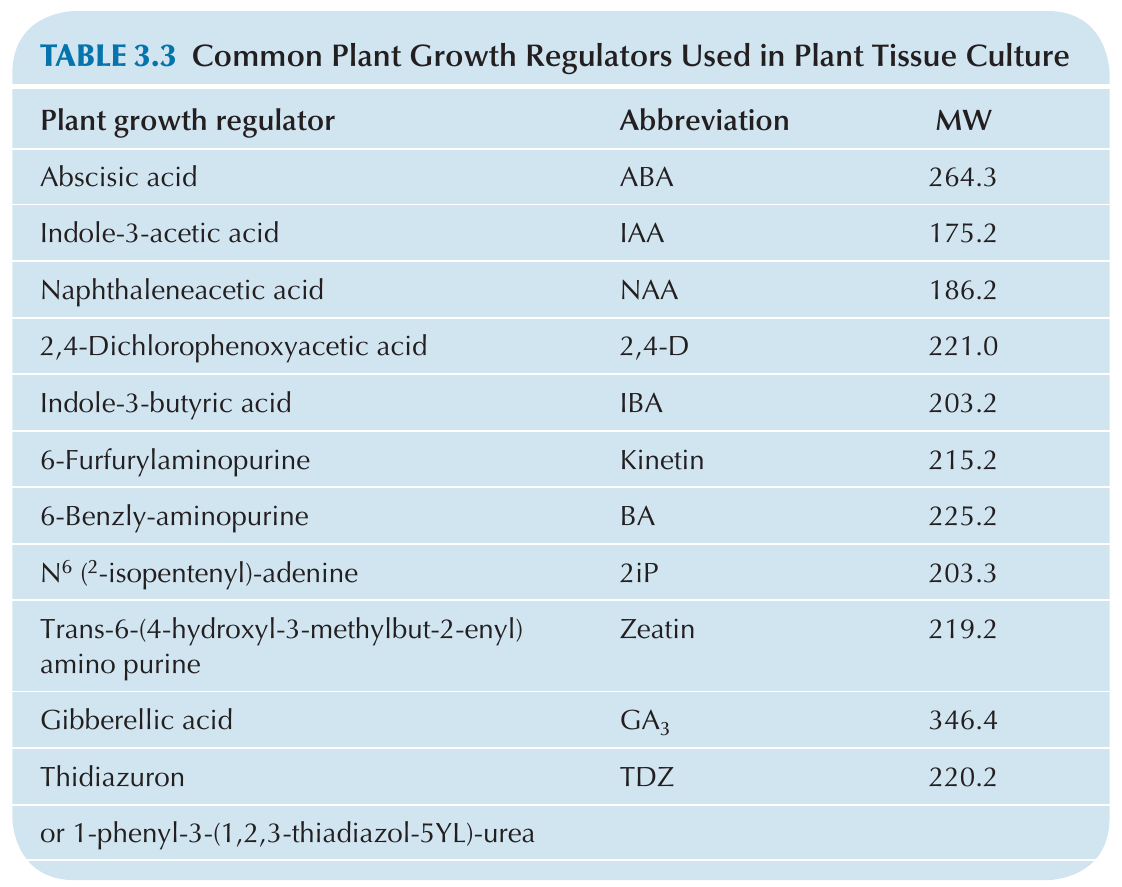
\includegraphics[width=0.9\linewidth]{../images/pgr_tissue_culture} \caption{Common plant growth regulators used in plant tissue culture}\label{fig:pgr}
\end{figure}

  \column{0.5\textwidth}

\begin{figure}
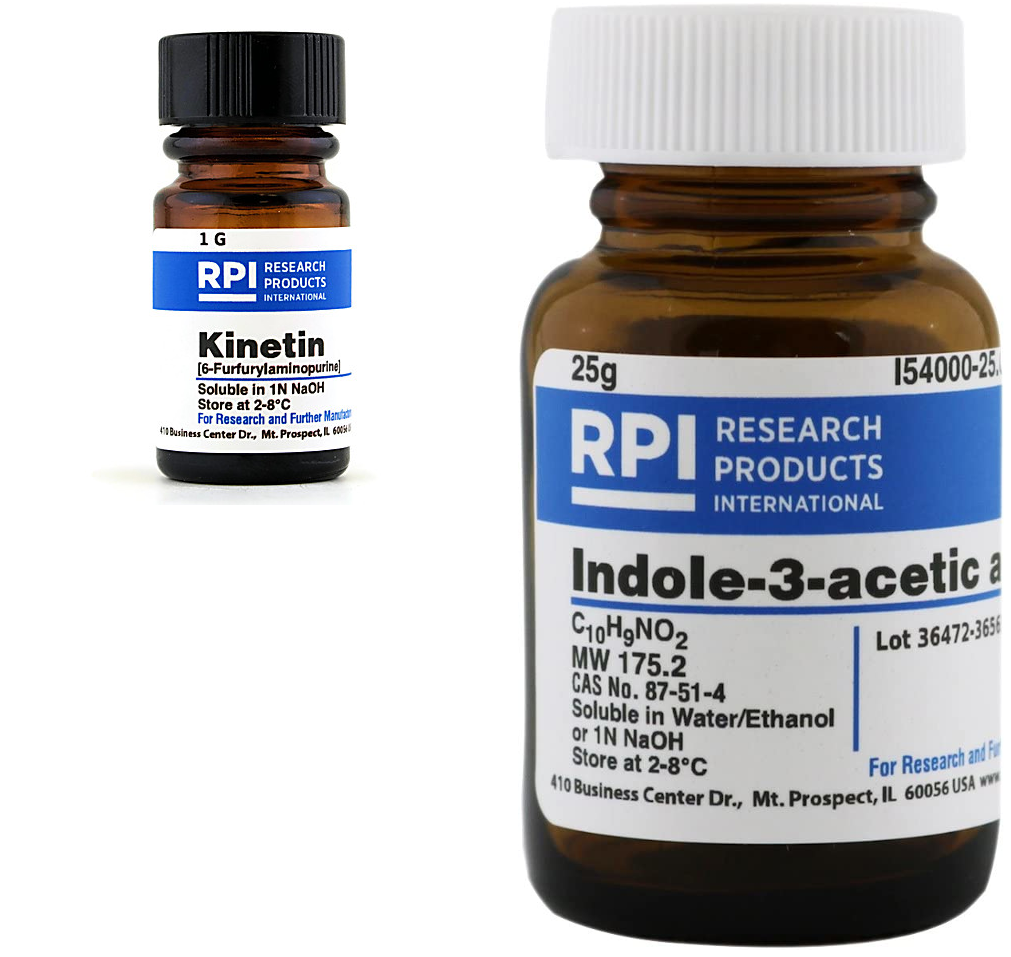
\includegraphics[width=0.6\linewidth]{../images/auxin-cytokinin} \caption{Commercial formulations of PGRs (Auxin and Cytokinin) used in tissue culture}\label{fig:auxin-cytokinin}
\end{figure}

\end{columns}
\end{frame}

\begin{frame}{PGRs}
\protect\hypertarget{pgrs}{}
\begin{itemize}
\tightlist
\item
  Type and concentration will vary according to the cell culture
  purpose. List is provided in Figure \ref{fig:pgr}.
\item
  Auxin (IAA, NAA, 2,4-D or IBA) is required by most plant cells for
  division and root initiation.
\item
  2,4-D is widely used for callus induction.
\item
  IAA, IBA and NAA are used for root induction.
\item
  Auxins can be dissolved either in alkali or in ethanol (latter is
  toxic to plants).
\item
  IAA stocks have a working duration of 1 weeks when kept away from
  light, they are thermostable, however.
\end{itemize}
\end{frame}

\begin{frame}{}
\protect\hypertarget{section-5}{}
\begin{itemize}
\tightlist
\item
  Cytokinins (kinetin, BA, zeatin and 2iP) promote cell division, shoot
  proliferation, and shoot morphogenesis.
\item
  Cytokinins are prepared in a fashion alike Auxins, except that 1 N HCL
  and a few drops of water are used to dissolve the crystals.
\item
  They can be stored for longer terms in the refrigerator and are
  thermostable.
\item
  Normally, gibberellin is infrequently used in plant cell culture due
  to callus growth and auxin induced adventitious root inhibition.
\end{itemize}
\end{frame}

\begin{frame}{}
\protect\hypertarget{section-6}{}
\begin{itemize}
\tightlist
\item
  Since stocks are highly susceptible to isomeric conversions, it should
  be made up fresh before addition to the medium by filter
  sterilization.
\item
  Abscisic acid (ABA), a plant hormone involved in leaf and fruit
  abscission and dormancy, is useful in embryo culture. Its stock
  solutions can be prepared in water. It is heat stable but light
  sensitive (conversion of cis to trans form in presence of light
  results in lesser biological activity).
\item
  Addition of ethylene biosynthetic inhibitors such as silver nitrate is
  beneficial.
\end{itemize}
\end{frame}

\begin{frame}{}
\protect\hypertarget{section-7}{}
\begin{figure}
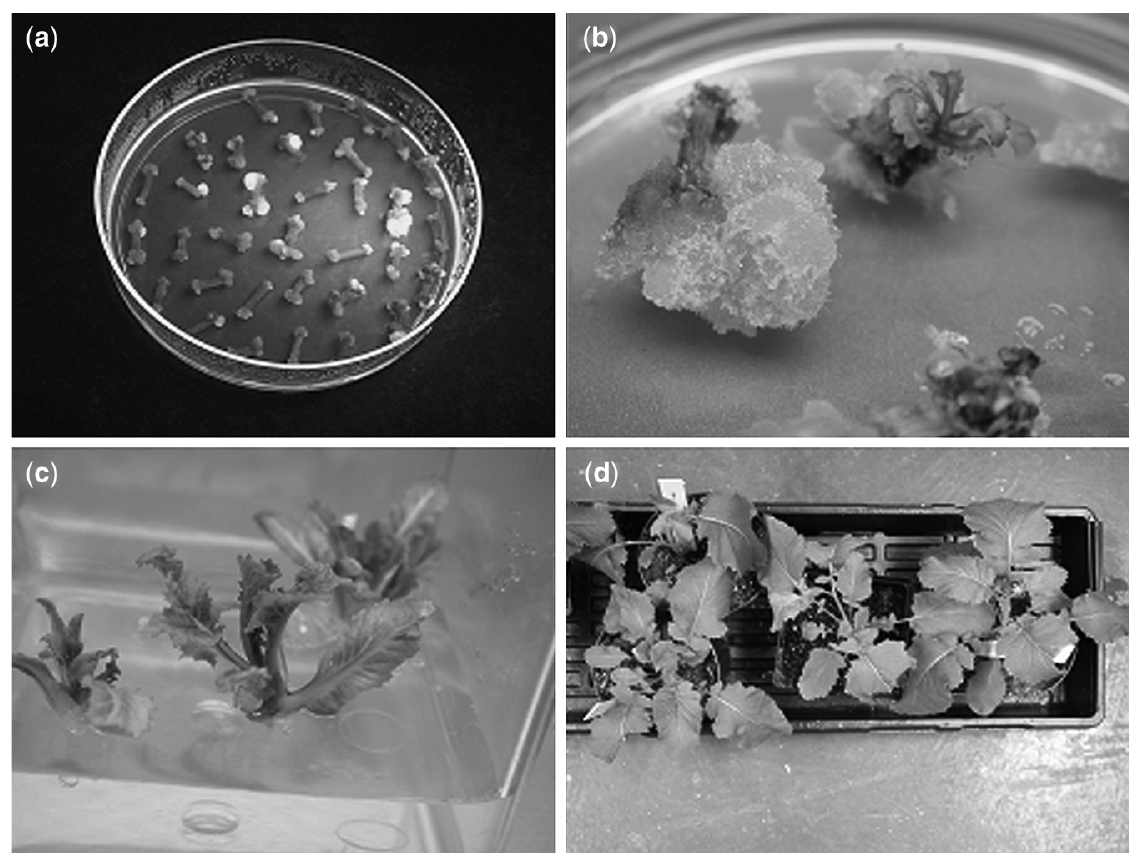
\includegraphics[width=0.45\linewidth]{../images/stages_of_tc} \caption{\textit{Brassica juncea} plants produced from hypocotyl explants. Shoots are produced when a combination of auxin and cytokinin is used.\newline (a) Callus from hypocotyl explants (note the green fluorescent protein fluorescent sectors on some of the calli); (b) shoots from callus; (c) shoots elongating; (d) whole plantlets transferred to soil.}\label{fig:stages-of-tc}
\end{figure}
\end{frame}

\begin{frame}{Vitamins}
\protect\hypertarget{vitamins}{}
\begin{itemize}
\tightlist
\item
  Catalytic functions in enzyme reactions.
\item
  Thiamine (B1), Nicotinic acid (B3) and Pyridoxine (B6) are added to
  cell culture media.
\item
  Stocks best stored in freezer.
\item
  10-ml aliquots used per liter of medium prepared.
\item
  Vitamin stocks used in these exercises contain 5 mg of nicotinic acid
  and 5 mg pyridoxine-hydrochloride per 100 ml of water.
\item
  The thiamine stock has 40 mg thiamine-hydrochloride in 1000 ml.
\end{itemize}
\end{frame}

\begin{frame}{}
\protect\hypertarget{section-8}{}
\begin{itemize}
\item
  \textbf{Common formulations}:

  \begin{itemize}
  \tightlist
  \item
    White (White 1963); in milligram-per-liter: 0.5 nicotinic acid, 0.1
    pyridoxine-hydrochloride, and 0.1 thiamine-hydrochloride;
  \item
    B5 Gamborg (Gamborg et al., 1976) with in milligram-per-liter
    medium: 100 inositol, 1.0 nicotinic acid, 1.0
    pyridoxine-hydrochloride, and 10.0 thiamine-hydrochloride;
  \item
    Murashige and Skoog (1962) with in milligram-per-liter medium: 100
    inositol, 0.5 nicotinic acid, 0.5 pyridoxine-hydrochloride, and 0.1
    thiamine-hydrochloride.
  \end{itemize}
\end{itemize}
\end{frame}

\begin{frame}{Carbohydrates}
\protect\hypertarget{carbohydrates}{}
\begin{itemize}
\tightlist
\item
  Green cells require carbohydrate source (as sucrose, glucose, fructose
  or even starch at 2-5\% (w/v)) until they are photosynthetically
  active.
\item
  Embryo and anther culture require higher levels of carbohydrates than
  that by protoplast culture.
\item
  Sugars undergo caramelization if autoclaved too long.
\end{itemize}
\end{frame}

\begin{frame}{Gelling agent}
\protect\hypertarget{gelling-agent}{}
\begin{itemize}
\tightlist
\item
  Provide stationary support
\item
  Can include filter paper, cotton, cheesecloth, vermiculite, special
  membrane rafts with a liquid medium.
\item
  Must include \alert{purified} agar.
\item
  Gelrite is transparent in appearance and is a polysaccharide produced
  from fermentation from \emph{Pseudomonas} sps.
\item
  Gelling should be done slowly in motion, while heating (in flask).
\item
  Medium is then dispensed in measured amounts in the culture container.
\item
  The agar can also be melted in the autoclave in a foil-capped
  Erlenmeyer flask for 15 min at \(121^\circ C\), 15 psi.
\end{itemize}
\end{frame}

\begin{frame}{Amino acids}
\protect\hypertarget{amino-acids}{}
\begin{itemize}
\tightlist
\item
  Important in morphogenesis.
\item
  L-forms are natural forms, which is also the only detectable form.
\item
  L-tyrosine can contribute to shoot initiation, L-arginine can
  facilitate rooting, L-serine can be used in microspore cultures to
  obtain haploid embryos.
\item
  Casein hydrolysate, an enzymatic digest of milk protein (caution: do
  not use the acid digest of milk proteins), was a common ingredient in
  many early media formulations as it provided a mixture of amino acids
  to enhance tissue response.
\end{itemize}
\end{frame}

\begin{frame}{Antibiotics}
\protect\hypertarget{antibiotics}{}
\begin{itemize}
\tightlist
\item
  Incorporation of bactericides and fungicides is to overcome
  contamination.
\item
  Generally not desired because they can be toxic to explants.
\item
  Transformaiton experiments using agrobacterium make it necessary to
  incorporate antibiotics (e.g.~Timentin, carbenicillin (500 mg/liter),
  cefotaxime (300 \(\mu\)g/ml)).
\item
  Should be added to medium after autoclaving.
\end{itemize}
\end{frame}

\begin{frame}{Natural complexes}
\protect\hypertarget{natural-complexes}{}
\begin{itemize}
\tightlist
\item
  Antioxidants, absorbents (charcoal), coconut endosperm, yeast extract,
  malt extract, tomato juice, etc.
\item
  Activated charcoal may be growth promoting (promotes morphogenesis and
  absorbs inhibitory compounds)
\end{itemize}
\end{frame}

\begin{frame}{Media pH}
\protect\hypertarget{media-ph}{}
\begin{itemize}
\tightlist
\item
  Agar will not gel properly above 6.0 (too firm gel).
\item
  pH naturally drops by 0.6-1.3 units after autoclaving and after cetain
  period of culturing.
\item
  Medium pH is adjusted with 1.0 or 0.1 N HCL or NaOH by using a
  medicine dropper
\end{itemize}
\end{frame}

\hypertarget{explant-preparation}{%
\section{Explant preparation}\label{explant-preparation}}

\begin{frame}{Explant age}
\protect\hypertarget{explant-age}{}
\begin{itemize}
\tightlist
\item
  Younger tissue is more responsive \emph{in vitro}.
\item
  Older tissues might not form callus.
\end{itemize}
\end{frame}

\begin{frame}{Season}
\protect\hypertarget{season}{}
\begin{itemize}
\tightlist
\item
  Spring season is appropriate time for good response in culture.
\item
  Tissues that have met dormancy requirements are useful.
\item
  Artificial chilling might also help enable break dormancy.
\item
  Contamination is associated with summer season.
\end{itemize}
\end{frame}

\begin{frame}{Explant size}
\protect\hypertarget{explant-size}{}
\begin{itemize}
\tightlist
\item
  Smaller the explant, the harder it is to culture.
\item
  Internal differences in hormone balance in the tissue can result in
  varying in vitro responses.
\end{itemize}
\end{frame}

\begin{frame}{Plant Quality}
\protect\hypertarget{plant-quality}{}
\begin{itemize}
\tightlist
\item
  Healthy, unstressed, virus free.
\end{itemize}
\end{frame}

\begin{frame}{Goal}
\protect\hypertarget{goal}{}
\begin{itemize}
\tightlist
\item
  If clonal propagation is the goal, then the explant will usually be a
  lateral or terminal bud or shoot.
\item
  For callus induction, pieces of the cotyledon, hypocotyl, stem, leaf,
  or embryo are usually used.
\item
  Excellent explants for callus induction are seedling tissues from
  aseptically germinated seeds or imma ture inflorescences.
\item
  Leaf tissue from the aseptically germinated seed is a good source of
  tissue for protoplast isolation.
\item
  To produce haploid plants or callus, the anther or pollen is cultured.
\end{itemize}
\end{frame}

\begin{frame}{Explant source}
\protect\hypertarget{explant-source}{}
\begin{columns}[T,onlytextwidth]

\column{0.5\textwidth}

\begin{figure}
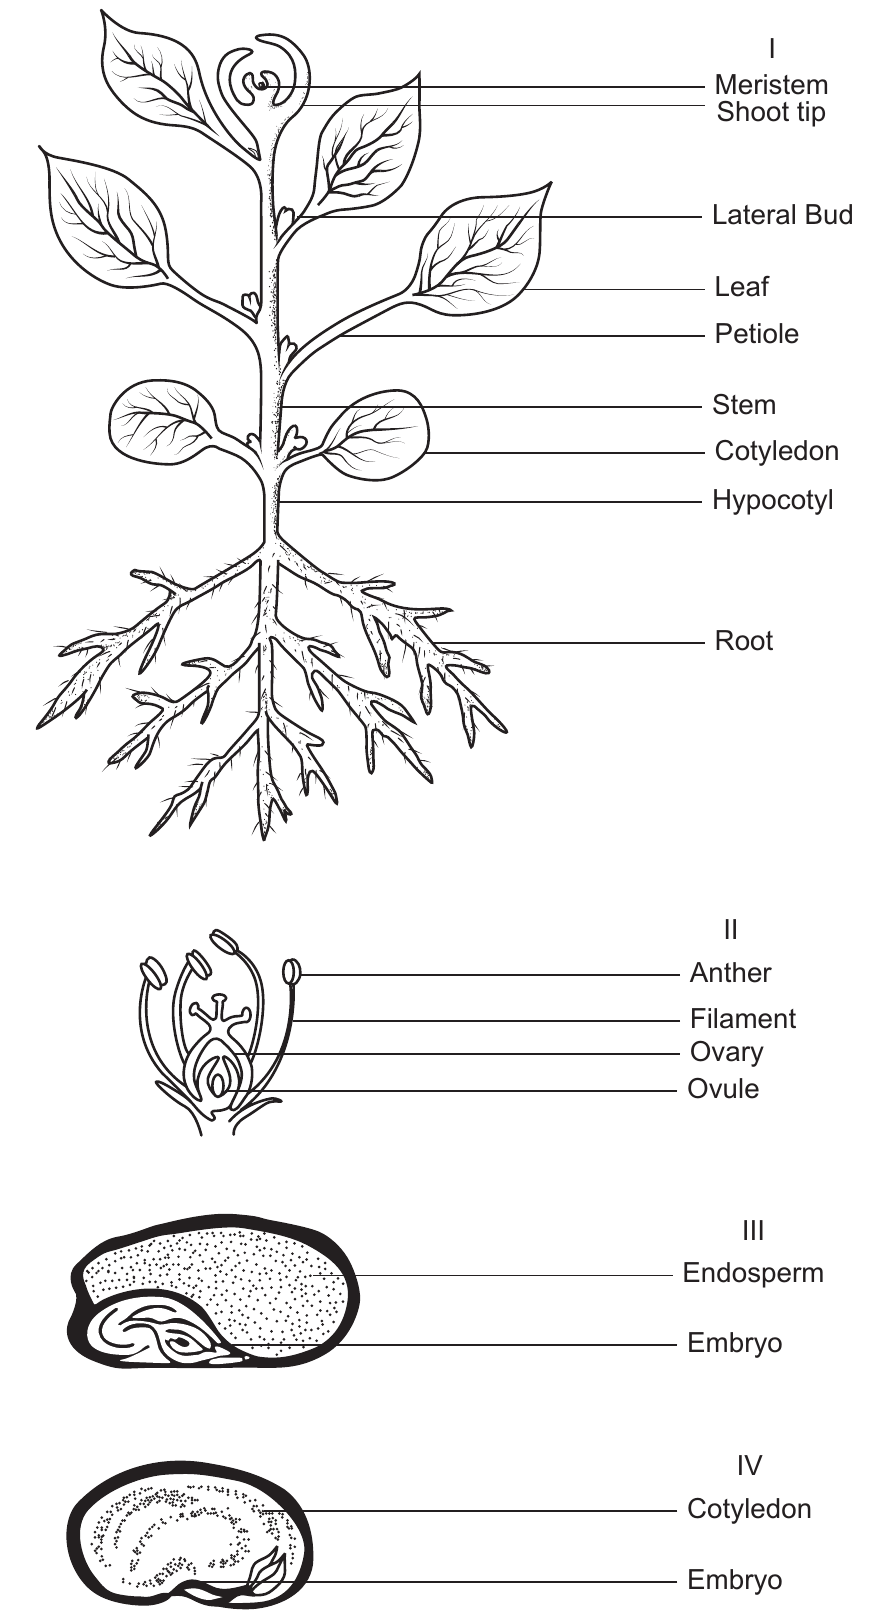
\includegraphics[width=0.45\linewidth]{../images/explant_sources} \caption{Schematic drawings (from top to bottom) of a plant, a flower, and monocotyledenous and dicotyldenous seeds indicate potential explant tissues.}\label{fig:explant-source}
\end{figure}

\column{0.5\textwidth}

\begin{figure}
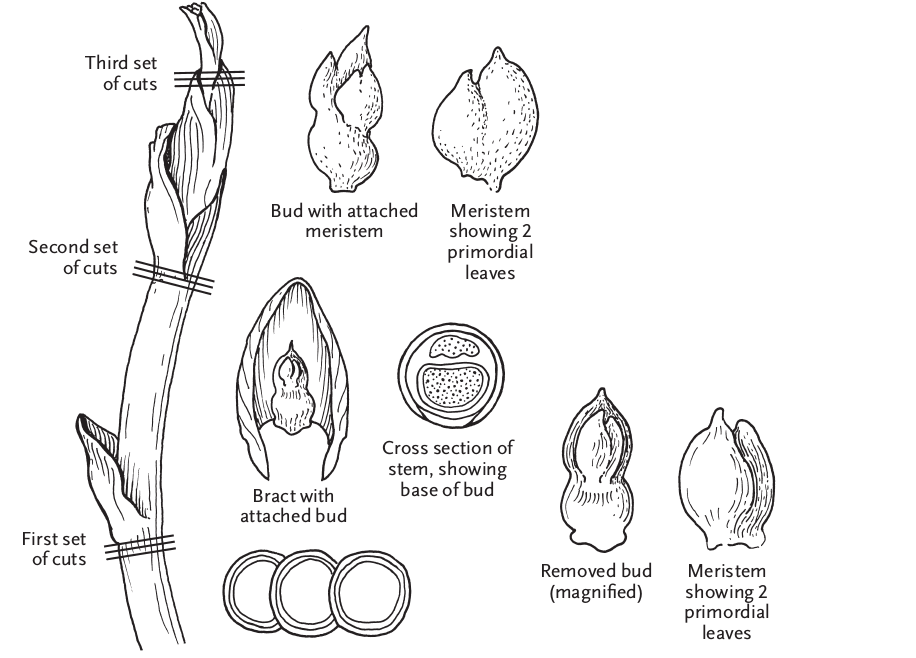
\includegraphics[width=0.9\linewidth]{../images/strawberry-meristem-generation} \caption{Strawberry (\textit{Fragaria} spp.) runner tip with 3 sites for obtaining meristematic tissue. When making each series of cuts, start at the bottom line and work up.}\label{fig:explant-source-strawberry}
\end{figure}

\end{columns}
\end{frame}

\begin{frame}{Other factors}
\protect\hypertarget{other-factors}{}
\begin{itemize}
\tightlist
\item
  Genotype: The ability to form regenerable callus in sorghum is
  heritable, and acted as a dominant trait (Ma et al., 1987). Also, rice
  regeneration is under control of both nuclear and cytoplasmic genes.
\item
  Aseptic technique
\item
  Asceptic germination of seeds
\item
  Contamination
\end{itemize}
\end{frame}

\hypertarget{processes-and-mechanism}{%
\section{Processes and mechanism}\label{processes-and-mechanism}}

\begin{frame}{Growth progression}
\protect\hypertarget{growth-progression}{}
\begin{figure}
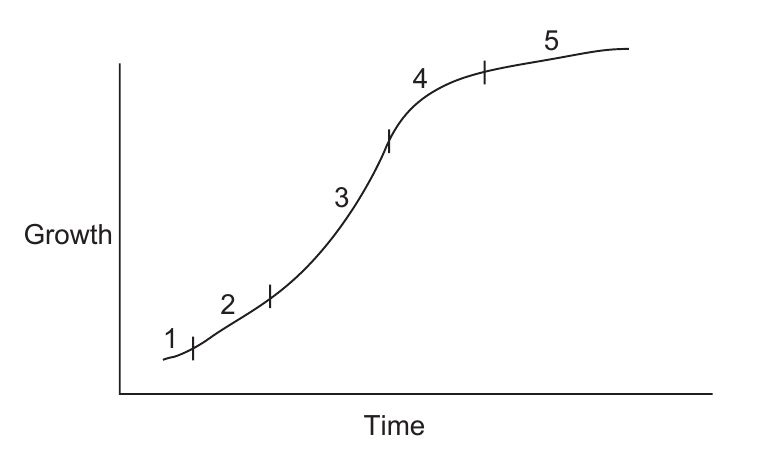
\includegraphics[width=0.4\linewidth]{../images/growth_curve} \caption{The rate of growth of callus tissue usually has five stages: (1) a lag phase in which cells prepare to divide; (2) a period of exponential growth in which cell division is maximal; (3) a period of linear growth in which division slows down and cells enlarge; (4) a period of decelerating growth; and (5) a stationary or no-growth period in which the number of cells is constant.}\label{fig:growth-curves}
\end{figure}
\end{frame}

\begin{frame}{Callus induction}
\protect\hypertarget{callus-induction}{}
\begin{itemize}
\tightlist
\item
  Explants may be an aseptically germinated seedling or
  surface-sterilized roots, stems, leaves, or reproductive structures.
\item
  \emph{Callus} is a wound tissue produced in response to injury. It is
  a proliferation of cells from the wounded or cut region of an explant.
  Callus is generally made up of friable, large, vacuolated cells that
  are highly differentiated, but are unorganized.
\item
  Callus can be hard and compact, and can contain regions of small
  meristematic cell clusters, which are undifferentiated cells competent
  to regenerate via somatic embryogeny or organ initiation.
\item
  Culture media (level of growth regulators) and conditions
  (temperature, light, solid vs.~agar media) are important for callus
  formation and development.
\item
  Culturing is maintained in dark condition at \(25-28^\circ\) C.
\item
  Medium generally has half-strength MS medium (for carrot) which is
  replaced by Gamborg's B5 medium after germination.
\end{itemize}
\end{frame}

\begin{frame}{Regeneration and morphogenesis}
\protect\hypertarget{regeneration-and-morphogenesis}{}
\begin{itemize}
\tightlist
\item
  Somatic embryogenesis (direct or indirect): plant or embryo is derived
  from a single somatic cell(not involved in embryo development)
\item
  First documented by Steward et al.~in 1958 with carrot cell suspension
  culture
\item
  Dividing cells undergoing embryogenesis first form a globular stage,
  then a heart stage, and then a torpedo stage, from which plantlets
  develop.
\item
  Shoot and roots are monopolar while somatic embryos are bipolar
\item
  Regeneration via somatic embryogenesis occurs in five steps:

  \begin{itemize}
  \tightlist
  \item
    initiation of embryogenic cultures,
  \item
    proliferation of embryogenic cultures,
  \item
    prematuration of somatic embryos,
  \item
    maturation of somatic embryos and,
  \item
    plant development on nonspecific media.
  \end{itemize}
\end{itemize}
\end{frame}

\begin{frame}{}
\protect\hypertarget{section-9}{}
\begin{itemize}
\tightlist
\item
  Initiation and proliferation occur on a medium rich in auxin, which
  induces differentiation of localized meristematic cells.
\item
  Once transferred to a medium with low or no auxin, these cells can
  then develop into mature embryos.
\item
  Germination occurs when it is mature enough to have functional root
  and shoot apices
\item
  Somatic embryogenesis follows organogenesis, during which organs and
  specialized tissues roots and shoots form.
\item
  Cell suspension culture may undergo organogenesis (through formation
  of callus) without embryogenesis.
\end{itemize}
\end{frame}

\begin{frame}{Cell culture pathway}
\protect\hypertarget{cell-culture-pathway}{}
\begin{figure}
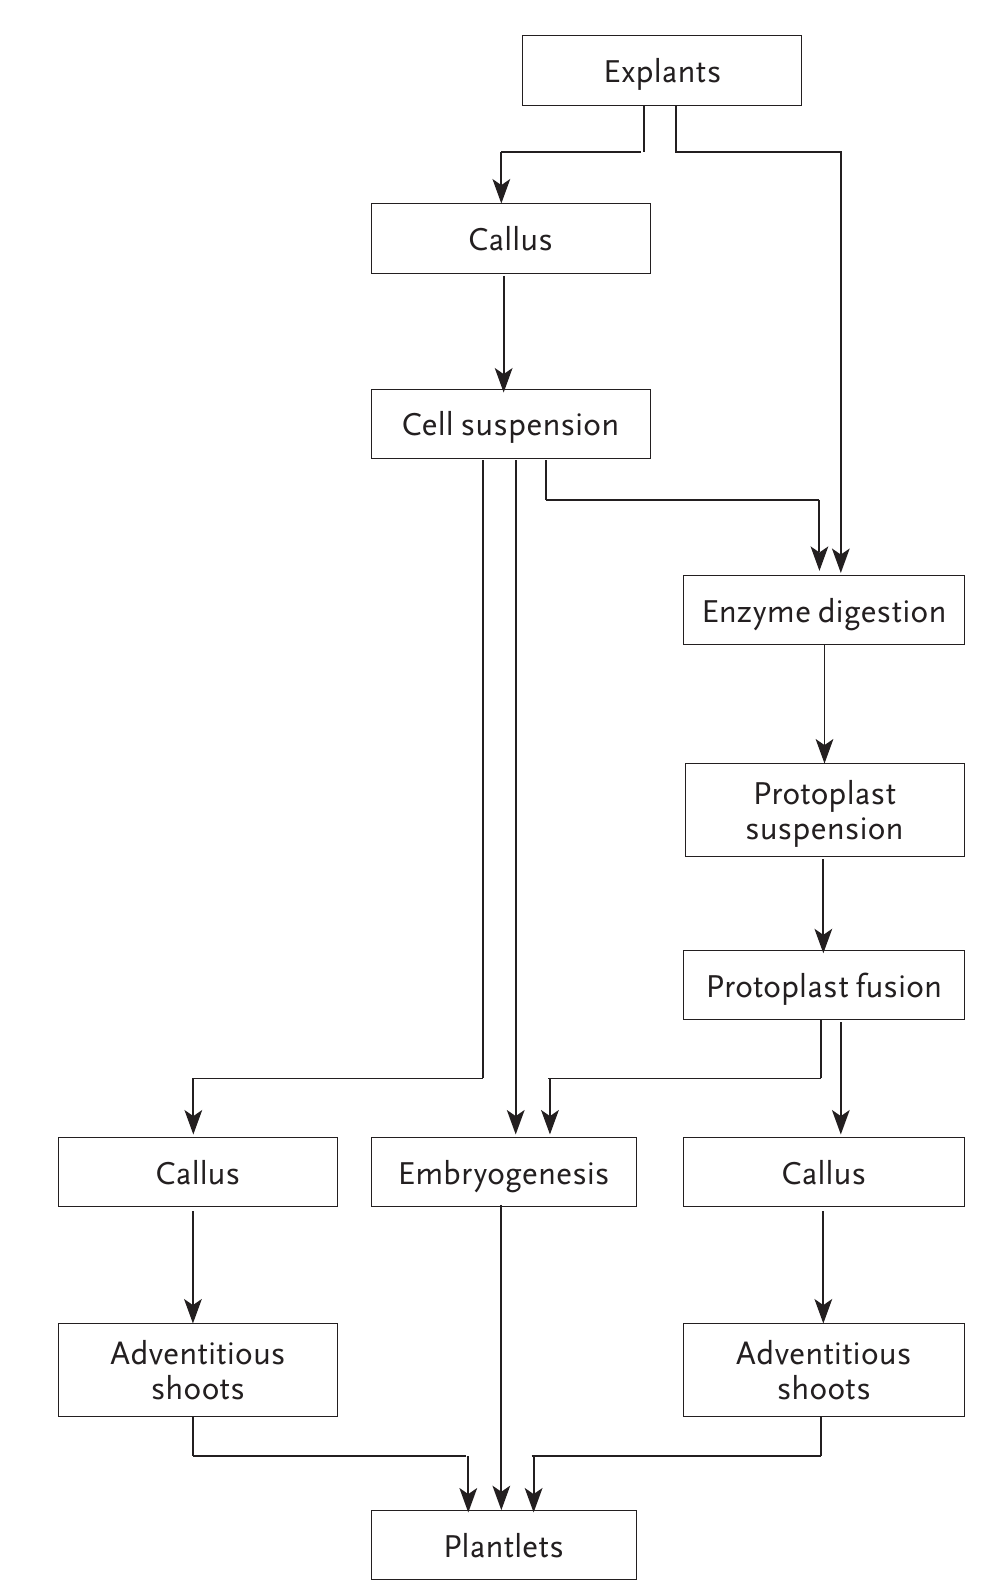
\includegraphics[width=0.28\linewidth]{../images/cell-culture-flowchart} \caption{A typical cell culture pathway.}\label{fig:cell-culture-pathway}
\end{figure}
\end{frame}

\hypertarget{bibliography}{%
\section{Bibliography}\label{bibliography}}

\hypertarget{references}{%
\subsection{References}\label{references}}

\end{document}
